\begin{enumerate}[label=\thechapter.\arabic*,ref=\thechapter.\theenumi]
\item A sinusoidal message signal having root mean square value of 4V and frequency of 1 kHz fed to a phase modulator with phase deviation constant 2 rad/volt. If the carrier signal is $c\brak{t} = 2\cos \brak{2\pi 10^6 t}$, the maximum instantaneous frequency of the phase modulated signal (rounded off to one decimal place) is \rule{1cm}{0.05mm} Hz. \hfill(GATE 2021 EC)\\
\solution\\
\iffalse
\let\negmedspace\undefined
\let\negthickspace\undefined
\documentclass[journal,12pt,twocolumn]{IEEEtran}
\usepackage{cite}
\usepackage{amsmath,amssymb,amsfonts,amsthm}
\usepackage{algorithmic}
\usepackage{graphicx}
\usepackage{textcomp}
\usepackage{xcolor}
\usepackage{txfonts}
\usepackage{listings}
\usepackage{enumitem}
\usepackage{mathtools}
\usepackage{gensymb}
\usepackage{comment}
\usepackage[breaklinks=true]{hyperref}
\usepackage{tkz-euclide} 
\usepackage{listings}
\usepackage{gvv}                                        
\def\inputGnumericTable{}                                 
\usepackage[latin1]{inputenc}                                
\usepackage{color}                                            
\usepackage{array}                                            
\usepackage{longtable}                                       
\usepackage{calc}                                             
\usepackage{multirow}                                         
\usepackage{hhline}                                           
\usepackage{ifthen}                                           
\usepackage{lscape}
\usepackage[center]{caption} % center the captions to figure

\newtheorem{theorem}{Theorem}[section]
\newtheorem{problem}{Problem}
\newtheorem{proposition}{Proposition}[section]
\newtheorem{lemma}{Lemma}[section]
\newtheorem{corollary}[theorem]{Corollary}
\newtheorem{example}{Example}[section]
\newtheorem{definition}[problem]{Definition}
\newcommand{\BEQA}{\begin{eqnarray}}
\newcommand{\EEQA}{\end{eqnarray}}
\newcommand{\define}{\stackrel{\triangle}{=}}
\theoremstyle{remark}
\newtheorem{rem}{Remark}
\begin{document}

\newcolumntype{M}[1]{>{\centering\arraybackslash}m{#1}}
\newcolumntype{N}{@{}m{0pt}@{}}

\bibliographystyle{IEEEtran}
\vspace{3cm}

\title{GATE 2022 BM 14 Q} 
\author{ee23btech11223 - Soham Prabhakar More% <-this % stops a space
}
\maketitle
\newpage
\bigskip

\renewcommand{\thefigure}{\theenumi}
\renewcommand{\thetable}{\theenumi}

\bibliographystyle{IEEEtran}

\textbf{Question:} $x\brak{t}$ is a real continuous-time signal whose magnitude frequency response
$\abs{X\brak{j\Omega}}$ is shown below. After sampling $x\brak{t}$ at 100 $rad.s^{-1}$, the spectral point P
is down-converted to \rule{1cm}{0.15mm} $rad.s^{-1}$ in the spectrum of the sampled signal.
\hfill{(GATE 2022 BM 14 Q)}
\begin{figure}[h!]
    \renewcommand\thefigure{1}
    \centering
    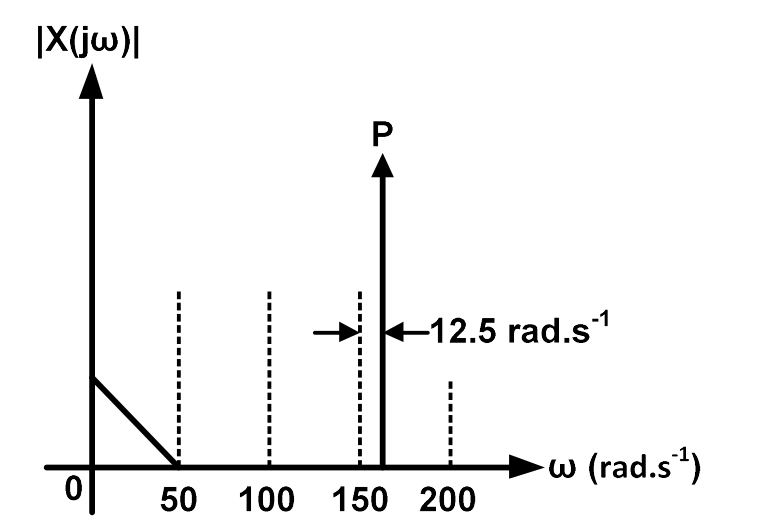
\includegraphics[width=\columnwidth]{2022/BM/14/figs/question.png}
    \caption[short]{Plot of $\abs{X\brak{j\omega}}$}
    \label{fig:2023.bm.14.img1}
\end{figure}

\solution
\fi
\begin{table}[ht]
    \renewcommand\thetable{1}
\begin{tabular}{|c|c|}
    \hline 
    \textbf{Parameter}&\textbf{Description} \\
    \hline
    $w\brak{t}$ & Sampling Function \\
    \hline
	$W\brak{j\omega}$ & Fourier Transform of $w\brak{t}$ \\
    \hline
    $x\brak{t}$ & Input Signal \\
    \hline
    $X\brak{j\omega}$ & Input Signal Frequency Spectrum \\
    \hline
    $x_s\brak{t}$ & Sampled Input Signal \\
    \hline
    $X_s\brak{j\omega}$ & Sampled Signal Frequency Spectrum \\
    \hline
\end{tabular}

\caption{Table of parameters}
\label{Table:1}


\end{table} \\
The sampling function is:
\begin{align}
    w(t) &= \sum_{k = -\infty}^{\infty}\delta\brak{t - \frac{2\pi k}{100}} \\
    W(j\omega) &= 100\sum_{k = -\infty}^{\infty}\delta\brak{j\brak{\omega - 100k}}
\end{align}
then the sampled function: 
\begin{align}
    x_s\brak{t} &= x\brak{t}w\brak{t} \\
    X_s\brak{j\omega} &= X\brak{j\omega} * W\brak{j\omega} \\
    X_s\brak{j\omega} &= \int_{-\infty}^{\infty}X\brak{j\theta}W\brak{j\brak{\omega - \theta}}d\theta \\
    X_s\brak{j\omega} &= 100\sum_{k = -\infty}^{\infty}\int_{-\infty}^{\infty}X\brak{j\theta}\delta\brak{j\brak{\omega - 100k - \theta}}d\theta \\
    X_s\brak{j\omega} &= 100\sum_{k = -\infty}^{\infty}X\brak{j\brak{\omega - 100k}} 
\end{align}
Thus, The down sampled point is at:
\begin{align}
    \omega &= \abs{162.5 - 100k}
\end{align}
where $k$ is the nearest integer to $\frac{162.5}{100}$, which is 2\\
Thus,
\begin{align}
    \omega = 37.5\,rad\,s^{-1}
\end{align}

\begin{figure}[h!]
    \renewcommand\thefigure{2}
    \centering
    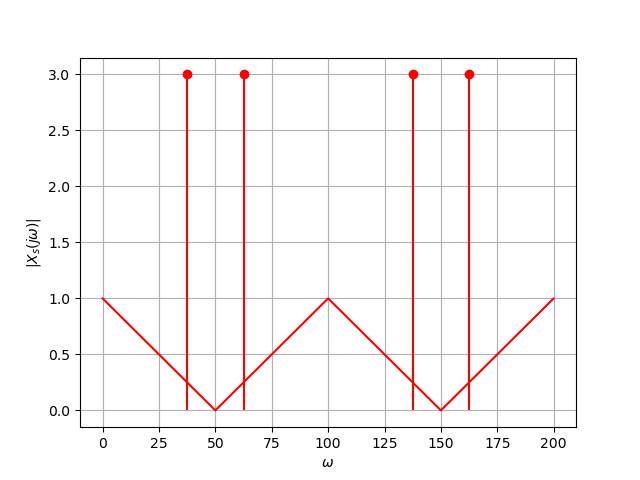
\includegraphics[width=\columnwidth]{2022/BM/14/figs/X_s.png}
    \caption[short]{Plot of $\abs{X_s\brak{j\omega}}$}
    \label{fig:2023.bm.14.img2}
\end{figure}

%\end{document}

\pagebreak
\item Two discrete-time linear time-invarient systems with impulse responses $h_1[n]=\delta[n-1]+\delta[n+1]$ and $h_2[n]=\delta[n]+\delta[n-1]$ are connected in cascade, where $\delta[n]$ is the Kronecker delta. The impulse response of the cascaded system is   \\
\begin{enumerate}[label=(\alph*)]
    \item $\delta[n-2]+\delta[n+1]$
    \item $\delta[n-1]\delta[n]+\delta[n+1]\delta[n-1]$
    \item $\delta[n-2]+\delta[n-1]+\delta[n]+\delta[n+1]$
    \item $\delta[n]\delta[n-1]+\delta[n-2]\delta[n+1]$
\end{enumerate} \hfill(GATE 2021 EE)\\
\solution
\input{2021/EE/7/gate7.tex}
\pagebreak
\item Consider a superheterodyne receiver tuned to 600 kHz. If the local oscillator feeds a 1000 kHz signal to the mixer, the image frequency (in integer) is \underline{\hspace{1cm}} kHz.
\hfill(GATE EC 2021)\\
\solution
\iffalse
\documentclass[journal,12pt,onecolumn]{IEEEtran}
\usepackage{cite}
\usepackage{amsmath,amssymb,amsfonts,amsthm}
\usepackage{algorithmic}
\usepackage{graphicx}
\usepackage{textcomp}
\usepackage{xcolor}
\usepackage{txfonts}
\usepackage{listings}
\usepackage{enumitem}
\usepackage{mathtools}
\usepackage{gensymb}
\usepackage{comment}
\usepackage[breaklinks=true]{hyperref}
\usepackage{tkz-euclide}
\usepackage{listings}
\usepackage{gvv}
\def\inputGnumericTable{}
\usepackage[latin1]{inputenc}
\usepackage{color}
\usepackage{array}
\usepackage{longtable}
\usepackage{calc}
\usepackage{multirow}
\usepackage{hhline}
\usepackage{ifthen}
\usepackage{lscape}

\newtheorem{theorem}{Theorem}[section]
\newtheorem{problem}{Problem}
\newtheorem{proposition}{Proposition}[section]
\newtheorem{lemma}{Lemma}[section]
\newtheorem{corollary}[theorem]{Corollary}
\newtheorem{example}{Example}[section]
\newtheorem{definition}[problem]{Definition}
\newcommand{\BEQA}{\begin{eqnarray}}
    \newcommand{\EEQA}{\end{eqnarray}}
\newcommand{\define}{\stackrel{\triangle}{=}}
\theoremstyle{remark}
\newtheorem{rem}{Remark}

\begin{document}
    
    \bibliographystyle{IEEEtran}
    \vspace{3cm}
    
    \title{Gate 2022 EC Q50}
    \author{EE23BTECH11212 - Manugunta Meghana Sai$^{*}$% <-this % stops a space
    }
    \maketitle
    \bigskip
    
    \renewcommand{\thefigure}{\theenumi}
    \renewcommand{\thetable}{\theenumi}
    
    \vspace{3cm}
    \textbf{Gate 2022 EC Q50} 
    
    Two linear time-invariant systems with transfer functions 
    \begin{align*}
    G_{1}\brak{s} = \frac{10}{s^{2} + s + 1} 
    \end{align*}
    and
    \begin{align*}
    G_{2}\brak{s} = \frac{10}{s^{2}+s\sqrt{10} +10}
    \end{align*}
    have unit step responses $y_{1}\brak{t}$ and $y_{2}\brak{t}$, respectively. Which of the following statements is/are true?
    \begin{enumerate}
    \item $y_{1}\brak{t}$ and $y_{2}\brak{t}$ have the same percentage peak overshoot.\\
    \item $y_{1}\brak{t}$ and $y_{2}\brak{t}$ have the same steady state values.\\
    \item $y_{1}\brak{t}$ and $y_{2}\brak{t}$ have the same damped frequency of oscillation.\\
    \item $y_{1}\brak{t}$ and $y_{2}\brak{t}$ have the same $2\%$ settling time.\\
    \end{enumerate}
    \solution
    \fi
    \begin{table}[h!]
 	\centering
 	\resizebox{6 cm}{!}{
 		\begin{tabular}{|c|c|c|}
	\hline
	\textbf{Parameter} &  \textbf{Description} & \textbf{value}\\[6pt]
	\hline
	$X_{1}\brak{s}$ & input & $\frac{1}{s}$ \\[6pt]
	\hline
	$X_{2}\brak{s}$ & input & $\frac{1}{s}$ \\[6pt]
	\hline
	$G_{1}\brak{s}$ & transfer function & $\frac{10}{s^{2} + s + 1} $ \\[6pt]
	\hline
	$G_{2}\brak{s}$ & transfer function & $\frac{10}{s^{2}+s\sqrt{10} +10} $ \\[6pt]
	\hline
	$y_{1}\brak{t}$ & unit step response & $-$\\[6pt]
	\hline
	$y_{2}\brak{t}$ & unit step response & $-$\\[6pt]
	\hline
	$\omega_{n}$ & natural frequency & $-$\\[6pt]
	\hline
	$\zeta$ & damping ratio & $-$\\[6pt]
	\hline 
	
\end{tabular}

 	}
 	\caption{Given Parameters}
 	\label{tab:msmECgate50tab1}
     \end{table} 
    The general second-order transfer function is given by:
    \begin{align}
    G\brak{s} = \frac{\omega_n^2}{s^2 + 2\zeta\omega_n s + \omega_n^2}
    \end{align}
    After comparing the coefficients of $G_{1}\brak{s}$ and $G_{2}\brak{s}$,
    \begin{table}[h!]
 	\centering
 	\resizebox{6 cm}{!}{
 		\begin{tabular}{|c|c|c|}
	\hline
	\textbf{Tranfer function} &  $\omega_{n}$ & $\zeta$\\[6pt]
	\hline
	$G_{1}\brak{s}$ & $1$ & $\frac{1}{2}$ \\[6pt]
	\hline
	$G_{1}\brak{s}$ & $\sqrt{10}$ & $\frac{1}{2}$ \\[6pt]
	\hline
\end{tabular}

 	}
 	\caption{Given Parameters}
 	\label{tab:msmECgate50tab2}
     \end{table} 
    as $\zeta = \frac{1}{2}$ is less than 1, the system is underdamped.
    \begin{align}
    Y\brak{s} &= X\brak{s} G\brak{s}\\
    &= \frac{1}{s} \brak{\frac{\omega_n^2}{s^2 + 2\zeta\omega_n s + \omega_n^2}}  
    \end{align}
    Applying inverse laplace transform,
    \begin{equation}
    y(t) = 1 - \frac{e^{-\zeta \omega_n t}}{1 - \zeta^2} \sin(\omega_d t + \phi)
    \label{eq:EC50msm}
    \end{equation}
    where $\omega_{d}$ is the damped frequency of oscillation.
    \begin{equation}
    \omega_{d} = \omega_{n}\sqrt{1 - {\zeta}^2}
    \label{eq:EC50msm2eq}
    \end{equation}
    The percentage peak overshoot $\brak{PO}$:
    \begin{equation}
    PO = \left( \frac{y_{\text{max}} - y_{\text{ss}}}{y_{\text{ss}}} \right) \times 100\%
    \label{eq:EC50msm1eq}
    \end{equation}
    $y_{\text{max}}$ is obtained by differentiating~\eqref{eq:EC50msm} with respect to time and equating it to zero, substituting the value in~\eqref{eq:EC50msm},
    \begin{align}
    y_{\text{max}} = 1 + \frac{1}{\sqrt{1-{\zeta}^2}}
    \end{align}
    $y_{\text{ss}}$ is obtained by final value theorem,
    \begin{align}
    y_{\text{ss}} &= \lim_{{s \to 0}} sY(s)\\
    &= \lim_{{s \to 0}} s\frac{\omega_n^2}{s^2 + 2\zeta\omega_n s + \omega_n^2} \frac{1}{s}\\
    &= 1
    \end{align} 
    Substituting the values of $y_{\text{max}}$ and $y_{\text{ss}}$ in~\eqref{eq:EC50msm1eq}, 
    \begin{align}
    PO = \frac{1}{\sqrt{1-{\zeta}^2}} \times 100\%
    \end{align}
    $y_{1}\brak{t}$ and $y_{2}\brak{t}$ have same $\zeta$, they have same percentage peak overshoot.So, option $\brak{1}$ is correct.\\
    The steady state value of $y\brak{t}$ is given by final value theorem:
    \begin{align}
    y_{1ss} &= \lim_{{s \to 0}} sY_{1}(s)\\
    &= \lim_{{s \to 0}} s \frac{10}{s^{2} + s + 1}  \frac{1}{s}\\
    &= 10\\
    y_{2ss} &= \lim_{{s \to 0}} sY_{2}(s)\\
    &= \lim_{{s \to 0}} s \frac{10}{s^{2}+s\sqrt{10} +10}  \frac{1}{s}\\
    &= 1
    \end{align} 
    as both the unit step responses have different steady state values, option $\brak{2}$ is incorrect.\\
    From~\eqref{eq:EC50msm1eq}, as $\omega_{n}$ is different for $y_{1}\brak{t}$ and $y_{2}\brak{t}$, they have different damped frequency of oscillation. Hence option $\brak{3}$ is incorrect.\\
    Settling time $T_s$:
    \begin{align}
    T_s = \frac{4}{\zeta \omega_n}
    \end{align}
    As, $\omega_{n}$ is different for $y_{1}\brak{t}$ and $y_{2}\brak{t}$, they have different $2\%$ settling time, Hence option $\brak{4}$ is incorrect.\\
    So, only option $\brak{1}$ is correct.   
%\end{document}


\pagebreak
\item A unity feedback system that uses proportional-integral (PI) control is shown in the figure.
 \begin{figure}[!ht]    
    \centering
\graphicspath{ {2021/EC/48/figs} }
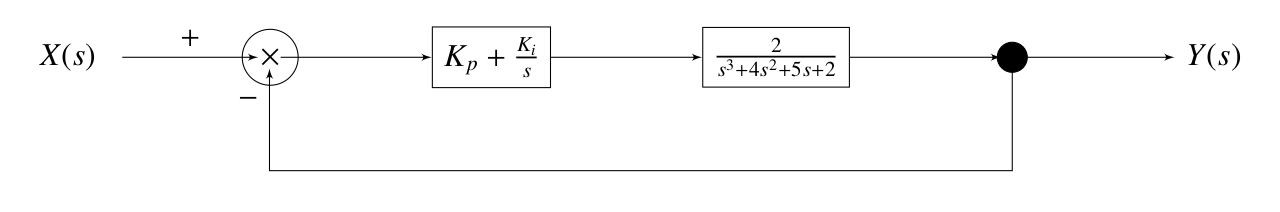
\includegraphics[width=\columnwidth]{figure_1}
\label{figure:ee25-gate4-graph}
\end{figure}
The stability of the overall system is controlled by tuning the PI control parameters $K_p$ and $K_i$. The maximum value of $K_i$ that can be chosen so as to keep the overall system stable or, in the worst case, marginally stable (\textit{rounded off to three decimal places}) is?
\hfill{(GATE EC 2021)}\\
\solution
\iffalse
\let\negmedspace\undefined
\let\negthickspace\undefined
\documentclass[journal,12pt,onecolumn]{IEEEtran}
\usepackage{cite}
\usepackage{amsmath,amssymb,amsfonts,amsthm}
\usepackage{algorithmic}
\usepackage{graphicx}
\usepackage{textcomp}
\usepackage{xcolor}
\usepackage{txfonts}
\usepackage{listings}
\usepackage{enumitem}
\usepackage{circuitikz}
\usepackage{mathtools}
\usepackage{gensymb}
\usepackage{comment}
\usepackage[breaklinks=true]{hyperref}
\usepackage{tkz-euclide} 
\usepackage{listings}
\usepackage{gvv}    
\usepackage{enumitem}
\usepackage{amsmath}
\def\inputGnumericTable{}                                 
\usepackage[latin1]{inputenc}                                
\usepackage{color}                                            
\usepackage{array}                                            
\usepackage{longtable}                                       
\usepackage{calc}                                             
\usepackage{multirow}                                         
\usepackage{hhline}                                           
\usepackage{ifthen}                                           
\usepackage{lscape}
\usepackage{tabularx}
\usepackage[italicdiff]{physics}
\usepackage{mathrsfs}
\usetikzlibrary{arrows,positioning}


\newtheorem{theorem}{Theorem}[section]
\newtheorem{problem}{Problem}
\newtheorem{proposition}{Proposition}[section]
\newtheorem{lemma}{Lemma}[section]
\newtheorem{corollary}[theorem]{Corollary}
\newtheorem{example}{Example}[section]
\newtheorem{definition}[problem]{Definition}
\newcommand{\BEQA}{\begin{eqnarray}}
\newcommand{\EEQA}{\end{eqnarray}}
\newcommand{\define}{\stackrel{\triangle}{=}}
\theoremstyle{remark}
\newtheorem{rem}{Remark}
\begin{document}
\bibliographystyle{IEEEtran}
\vspace{3cm}

\title{GATE:2021 - EC 48 }
\author{EE23BTECH11025 - Anantha Krishnan $^{}$% <-this % stops a space
}
\maketitle
\bigskip



\section{question}
A unity feedback system that uses proportional-integral (PI) control is shown in the figure.
 \begin{figure}[!ht]    
    \centering
\graphicspath{ {2021/EC/48/figs} }
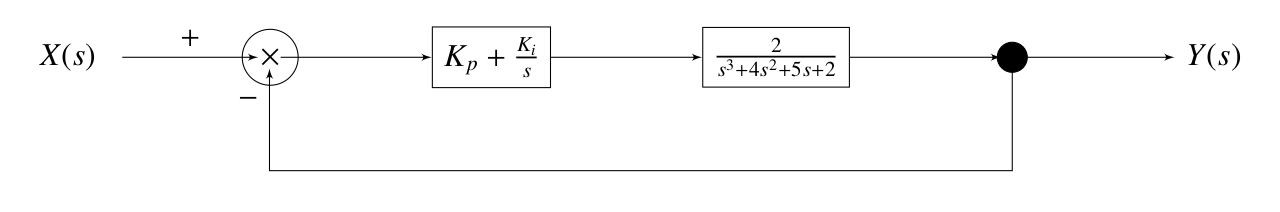
\includegraphics[width=\columnwidth]{figure_1}
\label{figure:ee25-gate4-graph}
\end{figure}
The stability of the overall system is controlled by tuning the PI control parameters $K_p$ and $K_i$. The maximum value of $K_i$ that can be chosen so as to keep the overall system stable or, in the worst case, marginally stable (\textit{rounded off to three decimal places}) is?
\hfill{(GATE EC 2021)}\\
 



\textbf{Solutions :}
\fi
    
\begin{table}[ht!]
\centering
\begin{tabular}{ |c|c|c| } 
 \hline
Symbols & Description & Values  \\
\hline
$P(s)$ & Plant transfer function & $\frac{2}{s^3+4s^2+5s+2}$ \\
 \hline
 $C(s)$ & PI controller transfer function &$K_p+\frac{K_i}{s}$\\
 \hline
$G(s)$ & Closed loop transfer function &$\frac{P(s)C(s)}{1+P(s)C(s)}$\\
 \hline
$Z$ & Number of zeroes with positive real part in $1+P(s)C(s)$ &?\\
 \hline
 $N$ & Total number of anticlockwise encirclements about $-1+0j$ in Nyquist plot & ?\\
\hline
$P$ & Number of poles with positive real part in $P(s)C(s)$ &?\\
\hline
\end{tabular}
\caption{Parameters, Descriptions, and Values}
\label{table:ee25-ec48-gate2021}
\end{table}




    From table \ref{table:ee25-ec48-gate2021}, the characteristic equation is given as:
    \begin{align}
        1+\brak{K_p+\frac{K_i}{s}}\brak{\frac{2}{s^3+4s^2+5s+2}} &= 0\\
        s^4+4s^3+5s^2+(2+2K_p)s+2K_i &=0 \label{eq:gate 2021 eq:4}
    \end{align}
    For the system to be stable, there must be no sign changes in the first column of the routh array for the above equation. From $\eqref{eq:gate 2021 eq:4}$
    \begin{align}
    \begin{array}{c|cccc}
        s^4 & 1 & 5 & 2K_i \\
        s^3 & 4 & (2 + 2K_p) & 0 \\
        s^2 & \frac{18-2K_p}{4} & 2K_i & 0 \\
        s^1 &  \frac{\brak{\frac{18-2K_p}{4}}\brak{2 + 2K_p}-8K_i}{\frac{18-2K_p}{4}} & 0 & 0\\
        s^0 & 2K_i &0 &0 \\
        \end{array}\\
        \end{align}
        \begin{align}
            \frac{18-2K_p}{4} &> 0\\
            \implies K_p &< 9 \label{eq:gate 2021 eq:1}\\
            \frac{\brak{\frac{18-2K_p}{4}}\brak{2 + 2K_p}-8K_i}{\frac{18-2K_p}{4}} &> 0\label{eq:gate 2021 eq:2}\\
        K_i &>0 \label{eq:gate 2021 eq:3}
    \end{align}
    For marginal stability, assuming 3 cases while maximising $K_i$ and checking if the above inequalities hold.
    \begin{enumerate}
        \item $K_p=9$\\
         \begin{align}
       \brak{\lim_{K_p\to9^-} \frac{\brak{\frac{18-2K_p}{4}}\brak{2 + 2K_p}-8K_i}{\frac{18-2K_p}{4}} > 0} &\cap \brak {K_i > 0}\\
       \brak{\lim_{K_p\to9^-} -8K_i > 0} &\cap \brak{{K_i > 0}}\\
  \implies K_p=9 , \forall K_i &\epsilon (\phi)
    \end{align}
    \item  $K_i=0$\\
    \begin{align}
        \brak{\brak{\frac{18-2K_p}{4}}\brak{2 + 2K_p} > 0}  \cap \brak{K_p < 9}\\
        \implies K_i=0 , \forall K_p \epsilon (-1 , 9)
    \end{align}
    \item $\frac{\brak{\frac{18-2K_p}{4}}\brak{2 + 2K_p}-8K_i}{\frac{18-2K_p}{4}} = 0$\\
        \begin{align}
            \brak{\frac{18-2K_p}{4}}\brak{2 + 2K_p} = 8K_i\\
             -K_p^2 +8K_p + 9 = 8K_i
        \end{align}
        Vertex ($K_p=4$) satisfies $\eqref{eq:gate 2021 eq:1}$:
        \begin{align}
            K_i &= 3.125 \forall (K_p = 4 ,K_i>0)
        \end{align}
          Based on the three cases for marginal stability, the maximum value of $K_i$ is $3.125$, for $K_p = 4$.\\
          \end{enumerate}

    \begin{enumerate}
        \item Verification by plotting roots of characteristic equation:\\
        If real part of atleast 1 root is equal to zero and for the rest are less than or equal to zero, then the system is marginally stable.
\begin{figure}    
    \centering
\graphicspath{ {2021/EC/48/figs} }
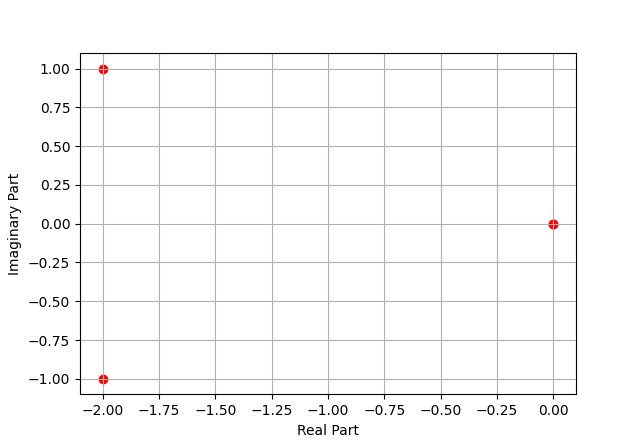
\includegraphics[width=\columnwidth]{graph_1}
\label{figure:ee25-gate4-graph1}
\caption{Location of roots for $k_i=0$,$k_p=-1$}
\end{figure}

\begin{figure}    
    \centering
\graphicspath{ {2021/EC/48/figs} }
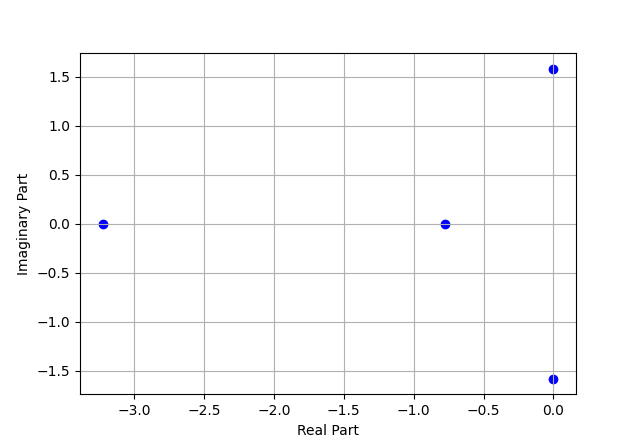
\includegraphics[width=\columnwidth]{graph_2}
\caption{Location of roots for $k_i=0$,$k_p=9$}
\label{figure:ee25-gate4-graph2}
\end{figure}

\begin{figure}    
    \centering
\graphicspath{ {2021/EC/48/figs} }
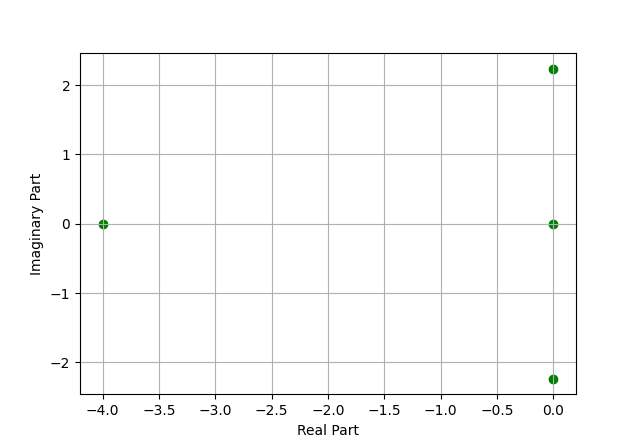
\includegraphics[width=\columnwidth]{graph_3}
\caption{Location of roots for $k_i=3.125$,$k_p=4$}
\label{figure:ee25-gate4-graph3}
\end{figure}

 \item Verification by Nyquist diagrams:\\
 From $\ref{table:ee25-ec48-gate2021}$, if $P=0$ and $-1+0j$ is neither bounded nor unbounded by the contour, then the system is marginally stable.
 For P:
 \begin{align}
     s^4+4s^3+5s^2+2s &= 0\\
     (s+1)^2(s+2) &= 0\\
     \implies P &= 0\\ 
     \implies Z &= N
 \end{align}
 
 
 \begin{figure}[!ht]    
    \centering
\graphicspath{ {2021/EC/48/figs} }
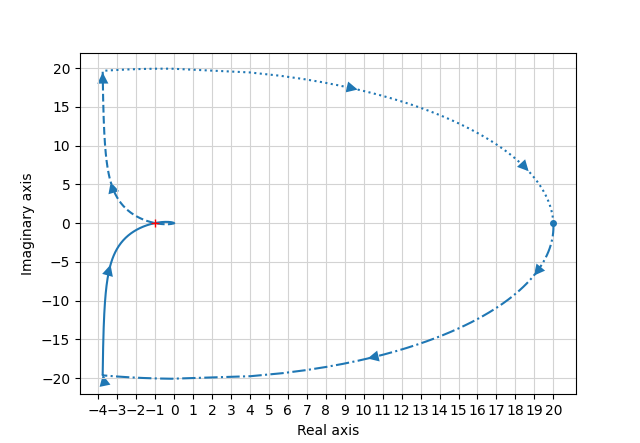
\includegraphics[width=\columnwidth]{plot_1}
\label{figure:ee25-gate4-nyquist1}
\caption{ Nyquist plot for $k_i=0$,$k_p=-1$}
\end{figure}

\begin{figure}[!ht]    
    \centering
\graphicspath{ {2021/EC/48/figs} }
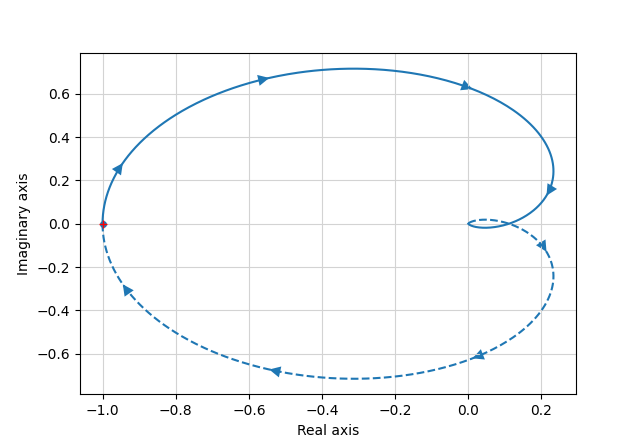
\includegraphics[width=\columnwidth]{plot_2}
\label{figure:ee25-gate4-nyquist2}
\caption{Nyquist plot for $k_i=0$,$k_p=9$}
\end{figure}

\begin{figure}[!ht]    
    \centering
\graphicspath{ {2021/EC/48/figs} }
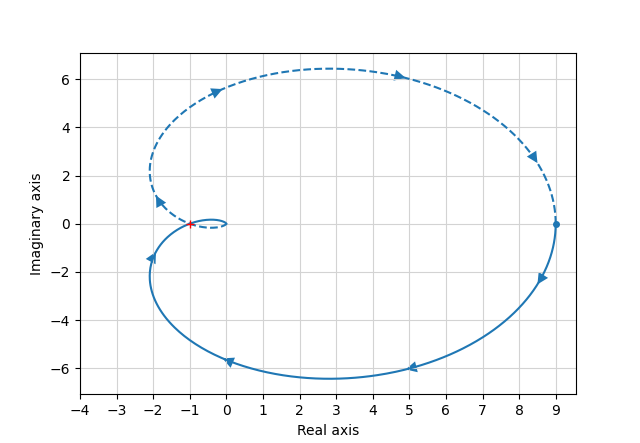
\includegraphics[width=\columnwidth]{plot_3}
\label{figure:ee25-gate4-nyquist3}
\caption{Nyquist plot for for $k_i=3.125$,$k_p=4$}
\end{figure}
     \end{enumerate}

  
   
    



\pagebreak
\end{enumerate}
